\section{Proprietà di un KGMS}

Un KGMS completo deve disporre di diversi requisiti, che elencheremo sulla base di tre categorie principali, descritte nei sottocapitoli 1.1.1, 1.1.2 ed 1.1.3

\subsection{Linguaggio e sistema per il reasoning}

Dovrebbe esistere un formalismo logico per esprimere fatti e regole, e di un engine per il reasoning che usa tale linguaggio che dovrebbe fornire le seguenti caratteristiche:
\begin{itemize}
	\item Sintassi semplice e modulare: Deve essere semplice aggiungere e cancellare fatti e nuove regole. I fatti devono coincidere con le tuple sul database.
	\item Alta potenza espressiva: Datalog è un buon punto di riferimento per il potere espressivo delle regole. Con una negazione molto lieve cattura PTIME.
	\item Calcolo numerico e aggregazioni: Il linguaggio deve essere arricchito con funzioni di aggregazione per la gestione di valori numerici.
	\item Probabilistic Reasoning: Il linguaggio dovrebbe essere adatto ad incorporare metodi di reasoning probabilistico e il sistema dovrebbe propagare probabilità o valori di certezza durante il processo di reasoning.
	\item Bassa complessità: Il reasoning dovrebbe essere tracciabile nella complessità dei dati. Quando possibile il sistema dovrebbe essere in grado di riconoscere e trarre vantaggio da set di regole che possono essere elaborate in classi di complessità a basso livello di spazio. 
	\item Rule repository, Rule management and ontology editor: È necessario fornire una libreria per l'archiviazione di regole e definizioni ricorrenti, ed un'interfaccia utente per la gestione delle regole.
	\item Orchestrazione dinamica: Per applicazioni più grandi, deve essere presente un nodo master per l'orchestrazione di flussi di dati complessi.
\end{itemize}

\subsection{Accesso e gestione dei Big Data}

\begin{itemize}
	\item Accesso ai Big Data: Il sistema deve essere in grado di fornire un accesso efficace alle sorgenti e ai sistemi Big Data. L'integrazione di tali tecniche dovrebbe essere possibile se il volume dei dati lo rende necessario.
	\item Accesso a Database e Data Warehouse: Dovrebbe essere concesso un accesso a database relazionali, graph databases, data warehouse, RDF stores ed i maggiori NoSQL stores. I dati nei vari storage dovrebbero essere direttamente utilizzabili come fatti per il reasoning.
	\item Ontology-based Data Access (OBDA): Consente ad un sistema di compilare una query che è stata formulata in testa ad un'ontologia direttamente all'interno del database.
	\item Supporto multi-query: Laddove possibile e appropriato, i risultati parziali di query ripetute dovrebbero essere valutati una volta e ottimizzati a questo proposito.
	\item Pulizia dei dati, Scambio e Integrazione: L'integrazione, la modifica e la pulizia dei dati dovrebbero essere supportati direttamente (attraverso il linguaggio).
	\item Estrazione di dati web, Interazione e IOT: Un KGMS dovrebbe essere in grado di interagire con il web mediante estrazione dei dati web rilevanti (prezzi pubblicizzati dai concorrenti) e integrandoli in database locali e scambiare dati con moduli e server web disponibili (API).
\end{itemize}

\subsection{Inserimento di codice procedurale e di terze parti}

\begin{itemize}
	\item Codice procedurale: Il sistema dovrebbe disporre di metodi di incapsulamento per l'incorporazione di codice procedurale scritti in vari linguaggi di programmazione e offrire un'interfaccia logica ad esso.
	\item Pacchetti di terze parti per il machine learning, text mining, NLP, Data Analytics e Data Visualization: Il sistema dovrebbe essere dotato di accesso diretto a potenti package esistenti per il machine learning, text mining, data analytics e data visualization. Esistono diversi software di terze parti per questi scopi, un KGMS dovrebbe essere in grado di utilizzare una moltitudine di tali pacchetti tramite opportune interfacce logiche.
\end{itemize}

\section{Architettura}

In Vadalog, il knowledge graph è organizzato come un repository, una collezione di regole Vadalog, a sua volta confezionate in librerie. \newline
Le regole e le librerie possono essere amministrate tramite un'interfaccia utente dedicata. \newline
Le fonti esterne sono supportate e gestite attraverso dei trasduttori, ovvero adattatori intelligenti che consentono un'interazione attiva con le fonti durante il processo di reasoning. \newline
Come indicato in figura~\ref{fig:architettura}, che rappresenta la nostra architettura di riferimento, la componente centrale di un KGMS è il suo motore di reasoning principale, che ha accesso ad un repository di regole. Sono stati raggruppati vari moduli che forniscono funzionalità pertinenti di accesso ai dati ed analisi. Come possiamo vedere ad esempio la possibilità di accedere a RDBMS utilizzando il linguaggio standard SQL, nonché l'accesso ai NoSQL Stores attraverso delle API, ecc...  \newpage \clearpage

\begin{figure}[h!]
	\centering
	\includegraphics[width=0.8\linewidth]{figure/architettura}
	\caption{Schema dell'architettura dell'Engine di Vadalog.}
	\label{fig:architettura}
\end{figure}

\subsection{Reasoning}

Il linguaggio Vadalog estende la famiglia di linguaggi Datalog$\pm $, che chiameremo anche Warded Datalog$\pm $, ovvero tutte le caratteristiche offerte dal linguaggio base, con la possibilità di utilizzare gli esiste nella testa delle regole. \newline
In particolare tale famiglia garantisce la \textit{wardedness}, ovvero limita l'interazione tra gli esiste (labeled null), garantendo che due esiste possano essere messi in join fra di loro, soltanto se tale elemento di join non viene proiettato in testa (Harmful Join), altrimenti potremmo trovarci nel non determinismo (NP), mentre utilizzando questa strategia viene garantita la P  (polinomiale).\newline
Ne parleremo in maniera più approfondita nel Capitolo 2. \newline \newline
In questa sezione viene mostrato il processo di reasoning, ovvero come il sistema sfrutta le proprietà chiave di Warded Datalog$\pm$. \newline
Il sistema Vadalog, fa un uso piuttosto alto di ricorsione, quindi è probabile che ci si ritrovi in un ciclo infinito all'interno del grafo di esecuzione (grafo contenente tutti i nodi per la ricerca della soluzione, partendo dai nodi di output ai nodi di input), si utilizza quindi una strategia di \textit{Termination Control}. \newline
Tale strategia, rileva ridondanza, ovvero la ripetizione di un nodo più volte, il prima possibile combinando il tempo di compilazione e tecniche a runtime. \newline
A tempo di compilazione, grazie alla wardedness, che limita l'interazione tra i labeled null, l'engine riscrive il programma in modo che i joins con specifici valori di labeled null non si verificheranno mai (Harmful Join elimination). \newline
A runtime, il sistema adotta una tecnica di potatura ottimale di ridondanza e rami che non terminano mai (per la ricorsione), questa tecnica è strutturata in due parti \textbf{detection} e \textbf{potatura}. \newline
Nella fase di detection, ogni volta che una regola genera un fatto che è simile ad uno dei precedenti, viene memorizzata la sequenza delle regole applicate, ovvero la provenienza. \newline
Nella fase di potatura, ogni volta che un fatto presenta la stessa provenienza di un altro e sono simili, il fatto non viene generato. \newline
Tale tecnica sfrutta a pieno le simmetrie strutturali all'interno del grafo, per scopi di terminazione i fatti sono considerati equivalenti, se hanno la stessa provenienza e sono originati da fatti simili tra loro. \newline

\subsection{L'architettura}

Il sistema Vadalog, per essere un KGMS efficace e competitivo, utilizza un'architettura in-memory, nel quale viene utilizzata la cache per velocizzare determinate operazioni, ed utilizza le tecniche descritte nel sottocapitolo 1.2.1, che garantiscono la risoluzione e la ridondanza. \newline
Da un insieme di regole Vadalog, viene generato un \textit{query plan} (cioè un grafo con un nodo per ogni regolae un arco ogni volta che la testa di una regola appare nel corpo di un'altra). \newline
Alcuni nodi speciali sono contrassegnati come input o output, quando corrispondono a set di dati esterni (input), o ad atomi per il reasoning (output), rispettivamente.
Il query plan è ottimizzato con diverse variazioni su tecniche standard, ad esempio \textit{push selections down} e \textit{push projections down} il più possibile vicino alla sorgente dati. \newline
Infine il query plan viene trasformato in un piano di accesso, dove i nodi di una generica regola vengono sostituiti dalle implementazioni appropriate per i corrispondenti operatori a basso livello (ad esempio selezione, proiezione, join, aggregazione, ecc...). \newline
Per ogni operatore sono disponibili un insieme di possibili implementazioni e vengono attivati in base a criteri di ottimizzazione comuni. \newline
In Figura~\ref{fig:query_plan_1} viene rappresentato un esempio di query plan di un semplice programma Vadalog.
\begin{figure}[h!]
	\centering
	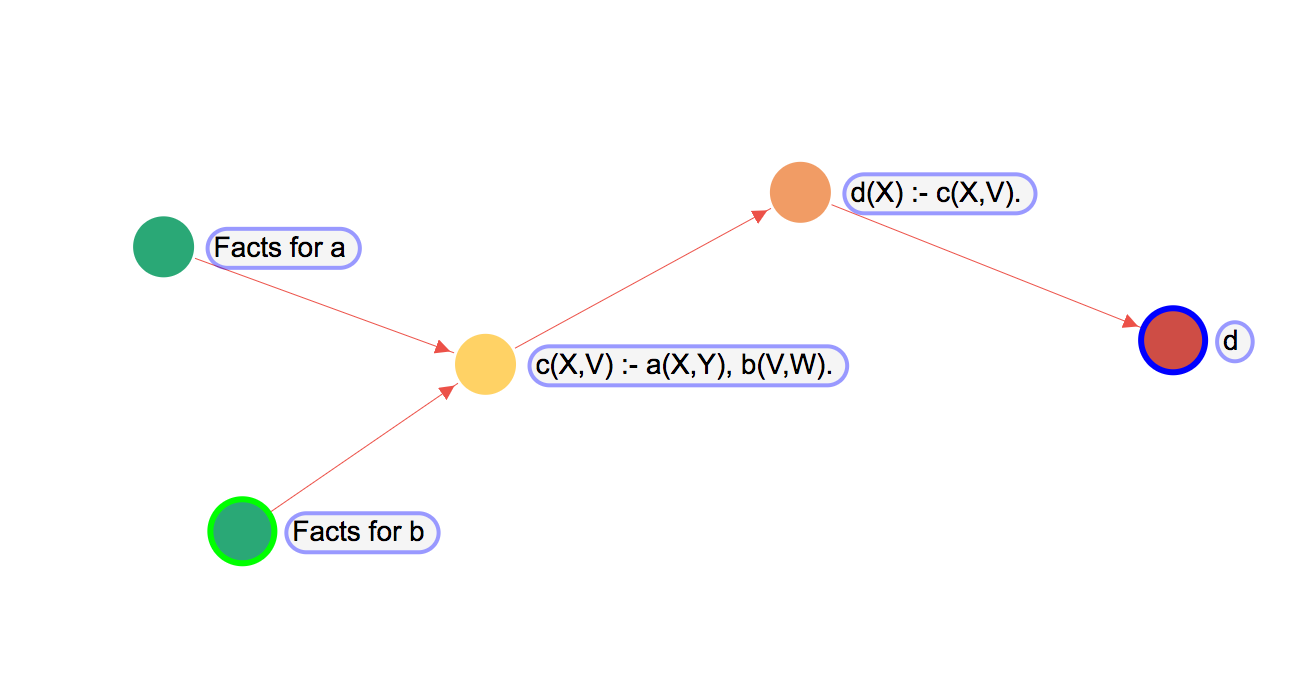
\includegraphics[width=0.8\linewidth]{figure/query-plan-ex1}
	\caption{Esempio di query plan.}
	\label{fig:query_plan_1}
\end{figure}

Il sistema Vadalog utilizza un approccio stream-based (o approccio a pipeline). Tale approccio~\cite{WIKI:STREAM} presume di avere i dati da elaborare organizzati in gruppi (stream) e che questi possano essere elaborati applicandone una serie di operazioni, spesso tali operazioni vengono elaborate tramite l'utilizzo di strutture a pipeline, e per ridurre i tempi vengono spesso utilizzate delle cache. \newline
Nel nostro sistema i fatti sono attivamente richiesti dai nodi di output ai loro predecessori e così via, fino ad arrivare ai nodi di input, che ricavano i fatti dalla sorgente dati. L'approccio stream è essenziale per limitare il consumo di memoria, in modo che il sistema è efficace per grandi volumi di dati. \newline
La nostra impostazione è resa più impegnativa dalla presenza di regole di interazione multipla e dalla presenza di ricorsioni. \newline
Gestiamo tali problemi utilizzando delle tecniche sui buffer, i fatti di ciascun nodo vengono messi in cache. \newline
La cache locale funziona particolarmente bene in combinazione con l'approccio basato sui stream, dato che i fatti richiesti da un successore possono essere immediatamente riutilizzati da tutti gli altri successori, senza avanzare ulteriori richieste. Inoltre questa combinazione realizza una forma di ottimizzazione multi-query, dove ogni regola sfrutta i fatti prodotti dagli altri ogni volta che risulta applicabile. \newline
Il problema principale è che in questo caso, se abbiamo a che fare con molti dati, la memoria rappresenta un limite, per limitarne l'occupazione, le cache locali vengono pulite con un \textit{Eager Eviction Strategy} che rileva quando un fatto è stato consumato da tutti i possibili richiedenti e quindi viene cancellato della memoria. \newline
I casi di cache overflow vengono gestiti ricorrendo alle scritture su disco (ad esempio LRU, LFU, ecc...). \newline
Le cache locali sono anche componenti funzionali fondamentali nell'architettura, poiché implementano in modo trasparente ricorsione e strategia di terminazione. \newline
Quindi, il meccanismo di stream è completamente agnostico sulle condizioni di terminazione, il suo compito è produrre dati per i nodi di output finché gli input forniscono fatti, è responsabilità delle cache locali rilevare la periodicità, controllare la terminazione e interrompere il calcolo ogni volta che ricorre un pattern noto. \newline
Possiamo vedere un esempio nella Figura~\ref{fig:architettura_1}, dove si nota all'interno del rettangolo bordato l'intero processo di stream, il nodo di output che richiede attivamente i fatti ai nodi intermedi (in questo caso un blocco contiene N nodi intermedi), e così via, fino ad arrivare ai nodi di input che chiedono i fatti alle sorgenti esterni (ad esempio Database, Datawarehouses, csv, ecc...). \newline
Nella parte superiore possiamo notare l'interazione tra il core e la cache, in questo caso si tratta di un'interazione periodica al fine di verificare ricorsioni cicliche per la strategia di terminazione. \newline
Ed infine è presente l'interazione tra il core ed il disco fisso, in questo caso essa avviene soltanto quando ci troviamo nel caso di cache overflow, in modo da fare il flush di tutti i dati della cache su disco fisso.\newpage \clearpage

\begin{figure}[h!]
	\centering
	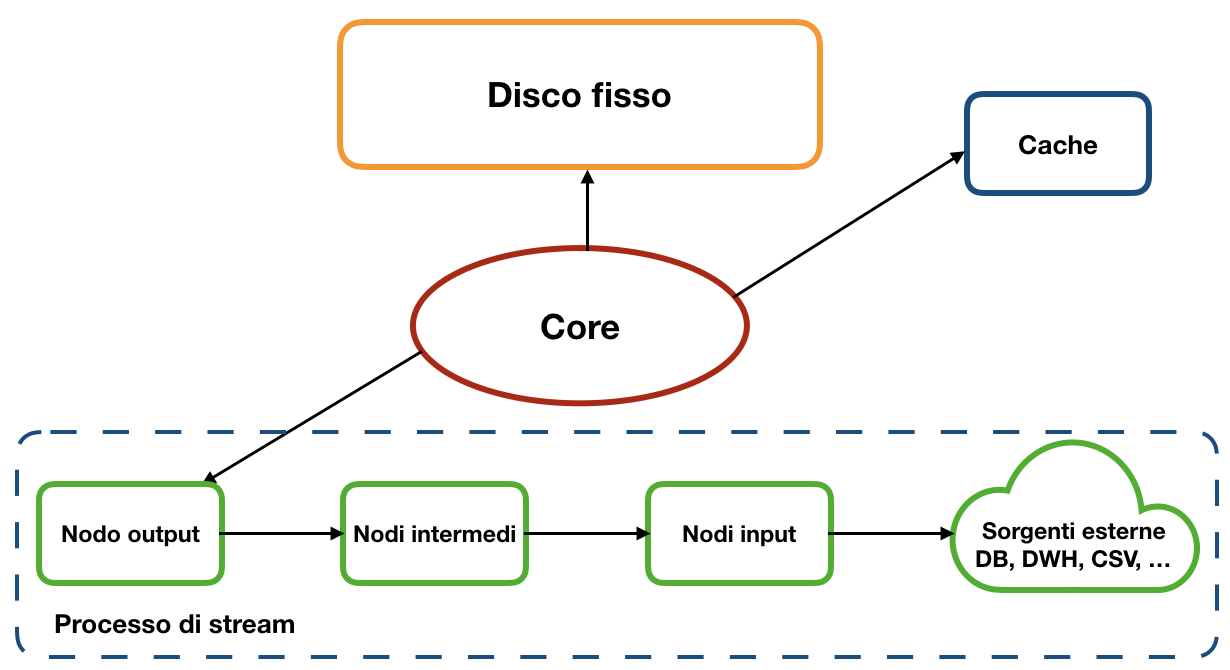
\includegraphics[width=0.8\linewidth]{figure/architettura-1}
	\caption{Funzionamento dell'architettura stream-based.}
	\label{fig:architettura_1}
\end{figure}

Per i join il sistema Vadalog adotta un estensione del Nested Loop Join, adatto per l'approccio stream-based ed efficiente in combinazione con le cache locali degli operandi. \newline
Tuttavia per garantire buone prestazioni, le cache locali sono migliorate dall'indicizzazione dinamica (a runtime) in memoria. In particolare, le cache associate ai join possono essere indicizzate mediante indici di hash creati a runtime, in modo da attivare un'implementazione ancora più efficiente di hash join.